\subsection{Постановка задачи}
Сформировать доменную модель для заданного текста.  Разработать тестовое покрытие для данной доменной модели.
\subsection{Описание предметной области}
\begin{quote}
	Легко, как балерина, Зафод вскочил на ноги и начал осматриваться. До самого горизонта во все стороны простиралась сплошная золотая поверхность. Она блестела, как... впрочем, этому невозможно подобрать сравнение, потому что ничто во Вселенной не блестит так, как планета из чистого золота.
\end{quote}
\subsection{UML-диаграмма}
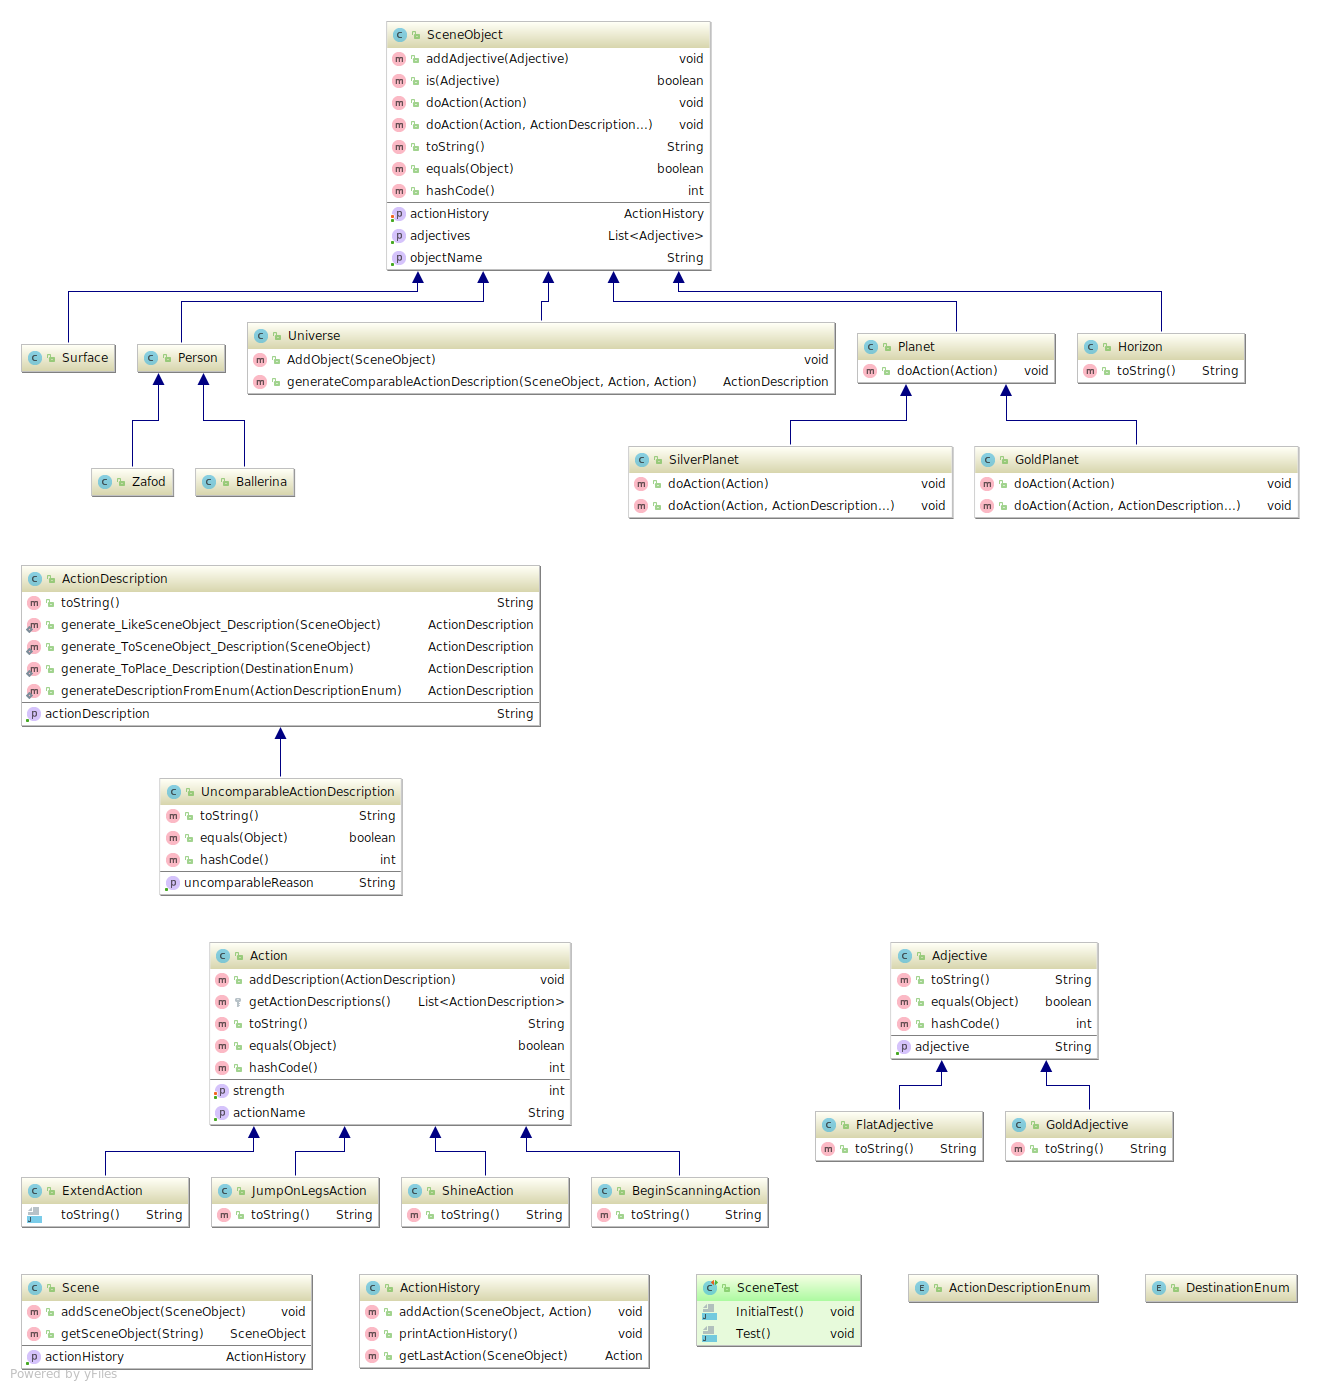
\includegraphics[scale=0.35]{scene_uml.png}
\subsection{Исходный код}
Не будем приводить полный исходный код, так как это не будет иметь смысла - очень много классов имеют схожий код внутри.
\subsubsection{SceneObject.java}
\lstinputlisting[language=java]{../src/main/java/testing/lab1/scene/SceneObject.java}
\subsubsection{Action.java}
\lstinputlisting[language=java]{../src/main/java/testing/lab1/scene/Action.java}
\subsubsection{ActionHistory.java}
\lstinputlisting[language=java]{../src/main/java/testing/lab1/scene/ActionHistory.java}
\subsubsection{Scene.java}
\lstinputlisting[language=java]{../src/main/java/testing/lab1/scene/Scene.java}
\subsection{Тесты}
% Приколы с юникодом, сорян
\begin{lstlisting}[language=java]
package testing.lab1.scene;

import org.junit.Test;

import static junit.framework.TestCase.assertNotNull;
import static junit.framework.TestCase.assertTrue;

public class SceneTest {

	@Test
	public void InitialTest() {
		Scene scene = new Scene();
		
		SceneObject obj1 = new SceneObject("obj1");
		SceneObject obj2 = new SceneObject("obj2");
		
		Action act1 = new Action("act1");
		Action act2 = new Action("act2");
		
		scene.addSceneObject(obj1);
		scene.addSceneObject(obj2);
		
		obj2.doAction(act1);
		obj1.doAction(act2);
		
		scene.getActionHistory().printActionHistory();
		
		assert(act1.getActionName().equals("act1"));

	}

	@Test
	public void Test() {
		//this has all the magic happening
		Scene scene = new Scene();
		
		//creating zafod and balerina
		Zafod zafod = new Zafod();
		Ballerina ballerina = new Ballerina();
		
		//this makes zafod log his actions to scene's log
		scene.addSceneObject(zafod);
		
		JumpOnLegsAction jump = new JumpOnLegsAction();
		zafod.doAction(jump, ActionDescription.generateDescriptionFromEnum(ActionDescriptionEnum.easily), ActionDescription.generate_LikeSceneObject_Description(ballerina));
		Action a = zafod.getActionHistory().getLastAction(zafod);
		assertTrue(a instanceof JumpOnLegsAction 
		&& a.getActionDescriptions().stream().anyMatch(
		ad -> ad.getActionDescription().equals("easily")));
		
		zafod.doAction(new BeginScanningAction());
		a = zafod.getActionHistory().getLastAction(zafod);
		assertTrue(a.getActionName().contains("scanning"));
		
		Surface surface = new Surface();
		scene.addSceneObject(surface);
		assertNotNull(scene.getSceneObject("surface"));
		
		Horizon horizon = new Horizon();
		ExtendAction extend = new ExtendAction();
		GoldAdjective ga = new GoldAdjective();
		FlatAdjective fa = new FlatAdjective();
		
		surface.addAdjective(ga);
		surface.addAdjective(fa);
		surface.doAction(extend, ActionDescription.generate_ToSceneObject_Description(horizon), ActionDescription.generate_ToPlace_Description(DestinationEnum.all_sides));
		assertTrue(
			surface.getActionHistory().getLastAction(surface)
			.getActionDescriptions().stream().anyMatch(
			ad -> ad.getActionDescription().contains(
			horizon.getObjectName()))
			&&
			surface.getActionHistory().getLastAction(surface)
			.getActionName().equals(
			new ExtendAction().getActionName())
			&&
			surface.is(new GoldAdjective())
			&&
			surface.is(new FlatAdjective())
		);
		
		
		//class universe with silver planet to compare shining strength to
		Universe uni = new Universe();
		SilverPlanet sp = new SilverPlanet();
		uni.AddObject(sp);
		
		
		ShineAction shine = new ShineAction();
		shine.setStrength(GoldPlanet.SHINING_STRENGTH);
		
		surface.doAction(shine, uni.generateComparableActionDescription(new GoldPlanet(), shine, new ShineAction()));
		assertTrue(surface.getActionHistory().getLastAction(surface).
		getActionDescriptions().stream().
		anyMatch(ad -> ad instanceof UncomparableActionDescription));
		
		//print out the whole story
		scene.getActionHistory().printActionHistory();
		
		//TODO: loads of more useful asserts
		assert(zafod.getObjectName().equals("Zafod"));
	}
}
\end{lstlisting}